\documentclass[tikz,border=5pt]{standalone}
\usepackage{amsmath,amssymb}
\usetikzlibrary{arrows.meta,positioning,trees}
\begin{document}
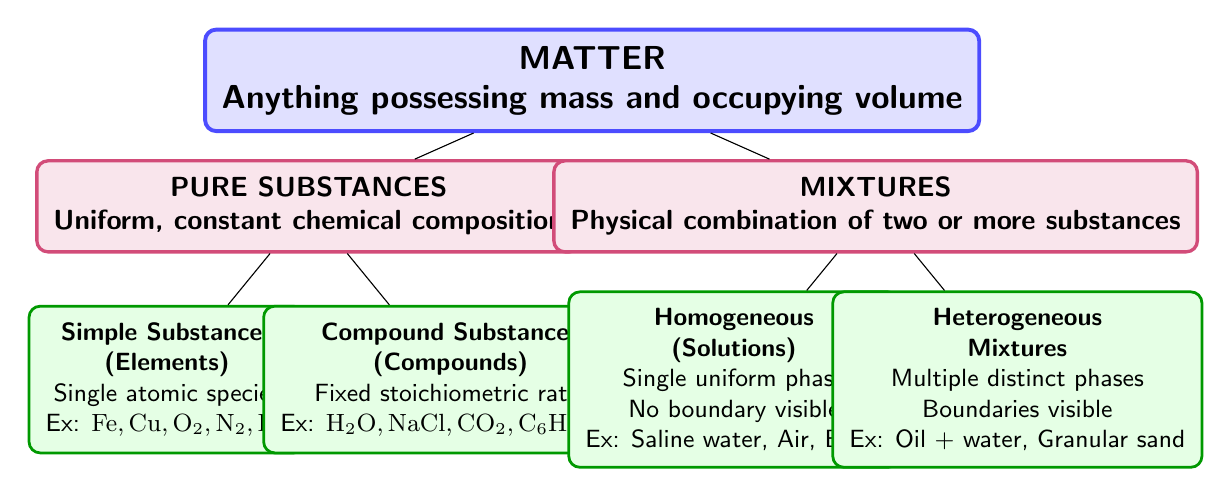
\begin{tikzpicture}[
  font=\sffamily,
  level 1/.style={sibling distance=7.2cm, level distance=1.6cm},
  level 2/.style={sibling distance=3.6cm, level distance=2.2cm},
  box/.style={draw=black!70, rounded corners=4pt, align=center, inner sep=6pt, line width=1pt},
  rootbox/.style={box, fill=blue!12, draw=blue!70, line width=1.4pt, font=\sffamily\bfseries\large},
  catbox/.style={box, fill=purple!10, draw=purple!70, line width=1.2pt, font=\sffamily\bfseries},
  subbox/.style={box, fill=green!10, draw=green!60!black, font=\sffamily\small}
]
  \node[rootbox] {\textbf{MATTER}\\Anything possessing mass and occupying volume}
    child {
      node[catbox] {\textbf{PURE SUBSTANCES}\\Uniform, constant chemical composition}
        child {
          node[subbox] {\textbf{Simple Substances}\\\textbf{(Elements)}\\Single atomic species\\Ex: $\mathrm{Fe, Cu, O_2, N_2, He}$}
        }
        child {
          node[subbox] {\textbf{Compound Substances}\\\textbf{(Compounds)}\\Fixed stoichiometric ratio\\Ex: $\mathrm{H_2O, NaCl, CO_2, C_6H_{12}O_6}$}
        }
    }
    child {
      node[catbox] {\textbf{MIXTURES}\\Physical combination of two or more substances}
        child {
          node[subbox] {\textbf{Homogeneous}\\\textbf{(Solutions)}\\Single uniform phase\\No boundary visible\\Ex: Saline water, Air, Brass}
        }
        child {
          node[subbox] {\textbf{Heterogeneous}\\\textbf{Mixtures}\\Multiple distinct phases\\Boundaries visible\\Ex: Oil + water, Granular sand}
        }
    };
\end{tikzpicture}
\end{document}
